%%%%%%%%%%%%%%%%%%%%%%%%%%%%%%%%%%%%%%%%%%
% if you want this to be a beamer project
% just rename this file to `main.tex` and
% and delete the original `main.tex`
%%%%%%%%%%%%%%%%%%%%%%%%%%%%%%%%%%%%%%%%%%
\documentclass[aspectratio=169]{beamer}
%\renewcommand{\thefootnote}{\fnsymbol{footnote}}
%\renewcommand*\footnoterule{\color{lhcb3}\rule{8cm}{.2mm}}
\setbeamersize{text margin left=4mm,text margin right=10mm}
\settowidth{\leftmargini}{\usebeamertemplate{itemize item}}
\addtolength{\leftmargini}{\labelsep}
\AtBeginEnvironment{frame}{\setcounter{footnote}{0}}
%\setbeamercolor{title separator}{fg=lhcb3, bg=lhcb3}
%\setbeamercolor{structure}{fg=lhcb3, bg=lhcb3}
%\setbeamercolor{page number in head/foot}{fg=lhcb3, bg=lhcb3}
%\usetikz{}

\usepackage{fontspec}
\usepackage{amsmath}
\usepackage{amssymb}
\usepackage{mathtools}

%Physics styles
\usepackage[
    math-style=ISO,
    bold-style=ISO,
    sans-style=italic,
    nabla=upright,
    partial=upright
]{unicode-math}

% numbers and units
\usepackage[
    %   locale=DE,
    separate-uncertainty=true,  % use \pm
    per-mode=symbol-or-fraction,
    binary-units=true,
    %per-mode=reciprocal,
    %output-decimal-marker=.,
]{siunitx}

% Fix missing micro sign with TL2017
\sisetup{
    math-micro=\text{μ},
    text-micro=μ,
    range-phrase = -,
    list-separator       = {, },
    list-final-separator = { und },
    range-units = single
}

% Positioning
\usepackage{float}
% Floats inside of section 
\usepackage[section, below]{placeins}
% same for Subsections 
\makeatletter
\AtBeginDocument{%
    \expandafter\renewcommand\expandafter\subsection\expandafter{%
        \expandafter\@fb@secFB\subsection
    }%
}
\makeatother
\floatplacement{figure}{htbp}
\floatplacement{table}{htbp}

% making caption look nice
\usepackage[
    labelfont=bf,
    font=small,
    width=0.9\textwidth,
]{caption}
\usepackage{subcaption}

% pictures
\usepackage{graphicx}

% Use _ in paths
\usepackage{grffile}

% tables
\usepackage{booktabs}

% optimizing look
\usepackage{microtype}
\usepackage[shortcuts]{extdash}

\usepackage{tikz}
\usepackage{tikz-feynman}
\usepackage{tikz-3dplot}

\setmainfont{Libertinus Serif}
\setsansfont{Libertinus Sans}
\setmonofont{Libertinus Mono}
\setmathfont{Libertinus Math}
\DeclareMathAlphabet{\mathcal}{OMS}{cmsy}{m}{n}

\usepackage[
    backend=biber,   % use modern biber backend
    autolang=hyphen, % load hyphenation rules for if language of bibentry is not
    % german, has to be loaded with \setotherlanguages
    % in the references.bib use langid={en} for english sources
    urldate=iso,%
    date=iso,%
    style=phys,%
    articletitle=false,biblabel=brackets,%
    chaptertitle=false,pageranges=false,%
    maxnames=2%
]{biblatex}

\usepackage{todonotes}
\presetkeys{todonotes}{inline}{}
%\setuptodonotes{color=lhcb3,size=\tiny}
\usepackage{xfrac}

\usetikzlibrary{patterns}
\usetikzlibrary{angles}
\usepackage{tabularx}

% quotation marks
\usepackage{csquotes}
\usepackage{slashed}
\usepackage{expl3}
\usepackage{xparse}
\usepackage{xcolor}
\usepackage{ifthen}
\usepackage{mleftright}
% my makros
% useful makros
\ExplSyntaxOn

\DeclareSIUnit\century{century}
\DeclareSIUnit\year{yr}

\makeatletter % allows me to use @
\NewDocumentCommand \showfont {} 
{encoding: \f@encoding{},
  family: \f@family{},
  series: \f@series{},
  shape: \f@shape{},
  size: \f@size{}
}
\NewDocumentCommand \symbfiftextbf {m}
{
    \ifthenelse{\equal{\f@series}{bx}\or\equal{\f@series}{b}}{\symbf{#1}}{#1}
}

\makeatother

\AtBeginDocument{
\let\ltext=\l
\RenewDocumentCommand \l {}
{
    \TextOrMath{ \ltext }{ \mleft }
}
\let\raccent=\r
\RenewDocumentCommand \r {}
{
    \TextOrMath{ \raccent }{ \mright }
}
}
\NewDocumentCommand \dif {}
{
    \mathinner{\symup{d}\mathchoice{\!}{\!}{}{} }
}

\ExplSyntaxOff
\NewDocumentCommand \tindex {mm}
{
    {#1_{\symup{#2}}}
}
\ExplSyntaxOn

\setlength{\delimitershortfall}{-1sp}
\DeclarePairedDelimiter{\abs}{\lvert}{\rvert}
\DeclarePairedDelimiter{\norm}{\lVert}{\rVert}
\DeclarePairedDelimiter\bra{\langle}{\rvert}
\DeclarePairedDelimiter\ket{\lvert}{\rangle}
\DeclarePairedDelimiterX\braket[2]{\langle}{\rangle}{#1 \delimsize\vert #2}

\NewDocumentCommand\xDeclarePairedDelimeter{mmm}
{%
\NewDocumentCommand#1{som}{%
\IfNoValueTF{##2}
    {\IfBooleanTF{##1}{#2##3#3}{\mleft#2##3\mright#3}}
{\mathopen{##2#2}##3\mathclose{##2#3}}%
}%
}
\xDeclarePairedDelimeter{\set}{\lbrace}{\rbrace}

\let\mysubsection=\subsection
\RenewDocumentCommand\subsection{m}
{
    \FloatBarrier
    \mysubsection{#1}
}

\NewDocumentCommand{\anti} {m}
{
    \overline{#1}
}

\AtBeginDocument{
    \RenewDocumentCommand \Re {} {\operatorname{Re}}
    \RenewDocumentCommand \Im {} {\operatorname{Im}}
}

\NewDocumentCommand{\mat}{m}{
    \symbf{#1}
}

\ExplSyntaxOff


% to use the LHCb colors, the same as in the plots
\definecolor{lhcb1}{HTML}{1f77b4}
\definecolor{lhcb2}{HTML}{ff7f0e}
\definecolor{lhcb3}{HTML}{2ca02c}
\definecolor{lhcb4}{HTML}{d62728}
\definecolor{lhcb5}{HTML}{9467bd}
\definecolor{lhcb6}{HTML}{8c564b}
\definecolor{lhcb7}{HTML}{e377c2}
\definecolor{lhcb8}{HTML}{7f7f7f}
\definecolor{lhcb9}{HTML}{bcbd22}
\definecolor{lhcb10}{HTML}{17becf}

\definecolor{mDarkBrown}{HTML}{604c38}
\definecolor{mDarkTeal}{HTML}{23373b}
\definecolor{mLightBrown}{HTML}{EB811B}
\definecolor{mLightGreen}{HTML}{14B03D}
\definecolor{vertexDarkGrey}{HTML}{23373b}
\definecolor{vertexLightGrey}{rgb}{0.833333333,0.8117647064,0.790196078}
\colorlet{vertexDarkRed}{red!70!black}
\colorlet{vertexLightRed}{vertexDarkRed!60!white}
\colorlet{vertexDarkGreen}{green!70!black}
\colorlet{vertexLightGreen}{vertexDarkGreen!50!white}
\colorlet{vertexDarkBlue}{blue!70!black}
\colorlet{vertexLightBlue}{vertexDarkBlue!50!white}


% Hyperlinks
\hypersetup{
    allbordercolors = vertexDarkGreen,
    unicode,        % Unicode in PDF-Attributen erlauben
    pdfusetitle,    % Titel, Autoren und Datum als PDF-Attribute
    pdfcreator={},  % ┐ PDF-Attribute säubern
    pdfproducer={}, % ┘
}
% erweiterte Bookmarks im PDF
\usepackage{bookmark} % look in there for more beamer settings 
\usetheme{metropolis} % Use metropolis theme

% Set language here
\usepackage[english]{babel}

\title{Discrete Fourier Transform of Images}
\date{\today}
\author{Ludwig Neste}
\institute{\colorbox{mDarkTeal}{
\includegraphics[width=.3\textwidth]{su_logo.pdf}}}

\addbibresource{references.bib}

\begin{document}

\begin{frame}
    \titlepage
\end{frame}

% \begin{frame}{Table of Contents}
%   \setbeamertemplate{section in toc}[sections numbered]
%   \tableofcontents[hideallsubsections]
% \end{frame}

\begin{frame}
    \frametitle{Fourier Transformation}

    An absolute integrable function
    \only<-2>{$f\!: \symbb{R}\to\symbb{C}$ }
    \only<3->{$f\!: \symbb{R}^{\color{mLightBrown} N}\to\symbb{C}$ }
    can be transformed to "frequency space":
    \only<-2>{
        \begin{align*}
            \symcal{F}  [f](\nu)
            =           \hat f(\nu) = & \int_{-\infty}^{\infty} f(x) e^{-i2\pi\nu x}        \dif x   \\
            \symcal{F}^{-1}[\hat f](x)
            =           f(x)        = & \int_{-\infty}^{\infty} \hat f(\nu) e^{i2\pi\nu x}  \dif \nu
        \end{align*}
    }
    \only<3->{
        \begin{align*}
            \symcal{F}  [f](\vec\nu)
            =           \hat f(\vec\nu) =  & \int_{\color{mLightBrown}\symbb{R}^N} f(x) e^{-i2\pi{\color{mLightBrown}\vec\nu \cdot \vec x}}        \dif{}^{\color{mLightBrown}N} x  \\
            \symcal{F}^{-1}[\hat f](\vec x)
            =           f(\vec x)        = & \int_{\color{mLightBrown}\symbb{R}^N} \hat f(\nu) e^{i2\pi{\color{mLightBrown}\vec\nu\cdot \vec x}}  \dif{}^{\color{mLightBrown}N} \nu
        \end{align*}
    }

    \begin{columns}
        \begin{column}[]{.5\textwidth}

            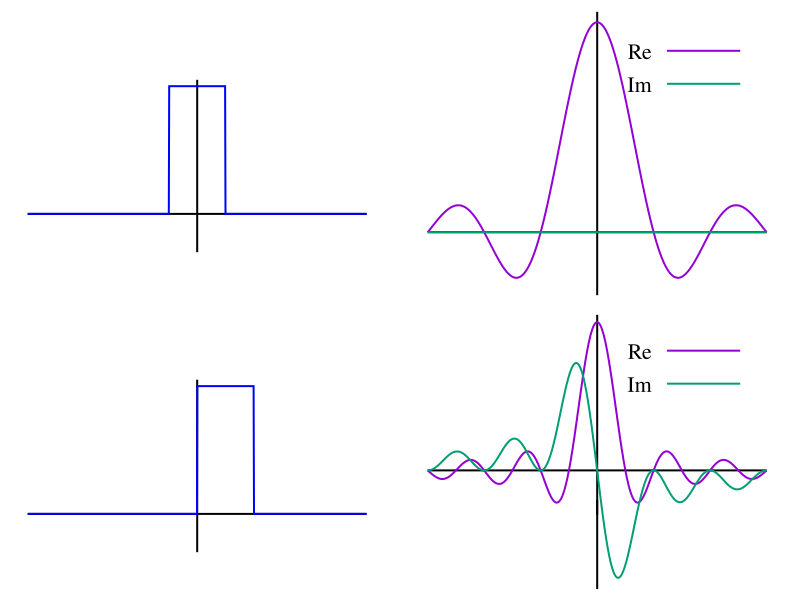
\includegraphics[trim=0 230 0 0, clip, width=\textwidth]{media/FT.png}
        \end{column}

        \begin{column}[]{.5\textwidth}

            \pause
            Important tool in physics:
            \begin{itemize}
                \item Solving differential equations
                \item Quantum mechanics: $\Psi(\vec p) = \symcal{F}[\Psi(\vec x)](\vec p)$
                \item Many more!
            \end{itemize}
        \end{column}
    \end{columns}


\end{frame}

\begin{frame}
    \frametitle{Discrete Fourier Transform}
    Let's model function, which is only nonzero at discrete values
    $0, 1, \dots, N-1$ with values proportional to $x_0, x_1, \dots, x_{N-1}$
    \begin{equation*}
        f(x) = \frac{1}{\sqrt N} \sum_{n=0}^{N-1} x_n\ \delta\left(x-{n}\right)
    \end{equation*}
    It's Fourier transform at points $0, 1/N, 2/N, \dots, N$ is the DFT of points $x_m$!
    \begin{equation*}
        \hat f\left(\frac{k}{N}\right)
        = \frac{1}{\sqrt N} \sum_{n=0}^{N-1} x_n e^{-i2\pi k \frac{n}{N}}
        = X_k
    \end{equation*}


\end{frame}

\begin{frame}
    \frametitle{(Inverse) Discrete Fourier Transform}
    \begin{equation*}
        X_k= \frac{1}{\sqrt N} \sum_{n=0}^{N-1} x_n e^{-i2\pi k \frac{n}{N}}
        \qquad \leftrightarrow \qquad
        x_k = \frac{1}{\sqrt N} \sum_{n=0}^{N-1} X_n e^{i2\pi k \frac{n}{N}}
    \end{equation*}
    \begin{columns}
        \begin{column}[]{.5\textwidth}
            \center
            \begin{tabular}{S[table-format=2.0] c<{\rightarrow} S[table-format=2.1] >{\hspace{-1em}}c<{\hspace{-.8em}} S[table-format=2.1]}
                4  &  & 44.1 & $+i$ & 0.0  \\
                8  &  & -2.4 & $+i$ & 14.8 \\
                15 &  & -9.8 & $+i$ & 9.1  \\
                16 &  & -9.8 & $+i$ & 0.0  \\
                23 &  & -9.8 & $-i$ & 9.1  \\
                42 &  & -2.4 & $-i$ & 14.8 \\
            \end{tabular}
        \end{column}
        \begin{column}[]{.5\textwidth}
            \begin{itemize}
                \item  $\symcal{F}^{-1}\left\{x_n\right\}
                          =\symcal{F}\left\{x_{N-n}\right\}
                          =\symcal{F}\left\{x_{n}^*\right\}^*$
                \item if $x_n$ real: $X_{k} = X^*_{N-k}$
            \end{itemize}
        \end{column}
    \end{columns}


\end{frame}
\begin{frame}{2D-DFT}

    \begin{equation*}
        X_{k,l} = \frac{1}{\sqrt{N_1N_2}}\sum_{n=0}^{N_1-1}\sum_{m=0}^{N_2-1}x_{n,m} \ e^{-i{2\pi}\ \left(\!\frac{kn}{N_1}+\frac{lm}{N_2}\right)}
        \qquad \leftrightarrow \qquad
        x_{k,l} = \frac{1}{\sqrt{N_1N_2}}\sum_{n=0}^{N_1-1}\sum_{m=0}^{N_2-1} X_{n,m} \ e^{i{2\pi}\ \left(\!\frac{kn}{N_1}+\frac{lm}{N_2}\right)}
    \end{equation*}

    These sums are separable:
    \begin{equation*}
        X_{k,l} =
        \frac{1}{\sqrt{N_1}}\sum_{n=0}^{N_1-1}e^{-i{2\pi}\frac{kn}{N_1}}
        \frac{1}{\sqrt{N_2}}\sum_{m=0}^{N_2-1}x_{n,m} \ e^{-i{2\pi}\frac{lm}{N_2}}
    \end{equation*}

    \color{mLightBrown}
    Perform a 2D-DFT by performing two 1D-DFT!
\end{frame}
\begin{frame}{Numerical Implementation}
    \begin{equation*}
        X_k= \frac{1}{\sqrt N} \sum_{n=0}^{N-1} x_n e^{-i2\pi k \frac{n}{N}}
    \end{equation*}
    Directly calculating this takes $N^2$ steps.
    Assuming $N$ is even, we can rewrite this as
    \begin{equation*}
        \begin{split}
            X_k &=\frac{1}{\sqrt N}
            \sum_{n=0}^{N/2-1} x_{2n} e^{-i\frac{2\pi}{N}2n k}+
            \frac{1}{\sqrt N}
            \sum_{n=0}^{N/2-1} x_{2n+1} e^{-i\frac{2\pi}{N}(2n+1) k}\\
            &= \frac{1}{\sqrt 2}
            \symcal{F}\left\{x_{2n}\right\}_k
            +\frac{1}{\sqrt 2}
            e^{-i\frac{2\pi}{N}k}\symcal{F}\left\{x_{2n+1}\right\}_k.
        \end{split}
    \end{equation*}
    We reduced the problem to about $2\cdot (N/2)^2=N^2/2$ steps.
\end{frame}
\begin{frame}{Fast Fourier Transform}
    \begin{itemize}
        \item If $N=2^p$, complexity is reduced via "Divide and Conquer" to $\symcal{O}(N\log N)$.
        \item One of the most important algorithms for modern signal processing
        \item Rediscovered and popularized by Cooley and Tukey in 1965\footnote{\fullcite{CTAlg}}
        \item Described in notes of Gauss 160(!) earlier
    \end{itemize}
\end{frame}
\begin{frame}{FFT of arbitrary size?}
    The Algorithm by Cooley-Tukey  works for every composite size $N=N_1\cdot N_2$

    What if $N$ is prime?
    \pause

    Then the set of numbers $G=\{0, 1, 2, \dots, N-1\}$ form a group with $\circ: G\times G\to G$
    \begin{equation*}
        a\circ b = a\cdot b\quad \symup{mod}\ N
    \end{equation*}
    DFT can then be expressed as a convolution. \emph{Rader's} Algorithm uses this to achieve $\symcal{O}(N\log N)$
\end{frame}
\begin{frame}{DCT}
    Let's stay real!
    \begin{align*}
        X_k =\frac{2c_k}{\sqrt N}\sum_{n=0}^{N-1}x_n \cos \left(\frac{\pi\left(2n+1\right)k}{2N} \right)
        \qquad \leftrightarrow & \qquad
        x_k
        =\frac{1}{\sqrt N}\sum_{n=1}^{N-1}c_n X_n \cos \left(\frac{\pi(2k+1)}{2N}n\right)
        \\
        \text{where }
        c_k =                  &
        \begin{cases}
            \frac{1}{\sqrt{2}} \quad & k=0           \\
            1                        & \text{ else }
        \end{cases}
    \end{align*}
    An efficient algorithm based on FFT\footnote{\fullcite{DCTUFFT}}:
    \begin{align*}
        \begin{rcases}
            x'_k       & = x_{2k}  \\
            x'_{N-1-k} & =x_{2k+1}
        \end{rcases}
        k=0,1, \dots, \frac{N}{2}-1
        \quad & \Rightarrow
        X_k =2 c_k
        \Re e^{i\pi\frac{k}{2N}}\symcal{F}^{-1}\left(\vec x'\right)_k
        \\
        x_{2k} =
        \Re \symcal{F}^{-1}\left\{c_lX_le^{i\frac{\pi l}{2N}}\right\}_k
        \qquad
              & x_{2k+1} = x_{2(N-1-k)}
    \end{align*}
\end{frame}
\section{Results}
All the implemented transforms where tested for correctness by comparing the output
of my implementation to other reference-implementations, like matlab's or scipy's.
The implementation was also tested for speed depending on the length of the input.
For a given input length the FFT algorithm was performed multiple times with random numbers
and the
runtime was measured and averaged. The number of times the algorithm was evaluated
was chosen, such that the uncertainty of the average was below \SI{10}{\nano\second}.
While the actual numbers will be more or less uninteresting, it is possible to see
the $\symcal{O}(N\log N)$ scaling for powers of 2, as shown in \autoref{fig:timesp2}.
Especially for higher-length input the scaling is fulfilled, but for short length
input there is too much overhead, and thus the numbers are not following $N\log N$ perfectly there.

\begin{figure}[htbp]
    \centering
    \includegraphics[width=\linewidth]{build/plots/times_p2.pdf}
    \caption{Runtime of the toy FFT algorithm in double-logarithmic-scaling depending on the length of the input sequence.
        Each random-number input was transformed multiple time and the results were averaged.
        The function $t(N)=c\times N\log N$ is fitted to the measurements, as we expect this scaling for
        input lengths in the form of $2^p$. }
    \label{fig:timesp2}
\end{figure}

For arbitrary sized input, the actual runtime of this algorithm depends heavily on
the number of two's in the prime-factor decomposition of the input-length.
In easier words: the FFT of 48 numbers should be roughly twice as fast as 56, even though
56 is the higher number.
The reason is 48 is divisible by 2 4 times ($48=2^4\cdot 3$), where 56 is only divisble by
2 3 times ($56=2^3\cdot 7$).
This is also clearly seen in the data, as \autoref{fig:times} shows.
\begin{figure}[htbp]
    \centering
    \includegraphics[width=.5\textwidth]{build/plots/times_lin_c.pdf}
    \caption{Averaged runtime of the implemented toy FFT algorithm on random numbers depending on the input length.
        A clear separation of the runtime scaling is seen. The data-points are colored
        depending on the number of times the input length is divisible by 2.}
    \label{fig:times}
\end{figure}


\subsection{Depicting the Fourier Space}
A digital image is nothing more than $N=h\cdot w\cdot C$ numbers $x_{k,l,c}$
\footnote{$k=0,\dots, h-1\quad l=0,\dots,w-1\quad c=0,\dots,C-1$}
between $0$ and $1$.
Where $w$ is the width, $h$ is the height and $C$ is the number of channels of the image.
There are a lot of different types of images out there, with different channel numbers and interpretation
of them (different color encodings, transparent images, etc.), but we will focus on the
case of grayscale $c=1$ or colored RGB $C=3$ pictrues.
The interpretation of the number in grayscale images is the illumination of the pixel ranging from $0=$~off~$=$~black
to $1=$~on~$=$~white.
In colored RGB images, we have three channels: Red (R), Green (G), Blue (B). Where we can light up each color seperately.
Because of how the eye works, we are able to trick the brain into perceiving most of the colors by just
mixing these three.
The numbers are usually not stored as floating point numbers, but as unsigned integers, most commonly 8-bit unsigned integers.
This means that 1 is stored as 255 and all the numbers are mapped in an equally spaced fashion.
If we have multiple channels, we will Fourier transform each channel separately
\begin{equation}
    X_{k,l,c} = \frac{1}{\sqrt{hw}}\sum_{n=0}^{h-1}\sum_{m=0}^{w-1}x_{n,m,c} \ e^{-i{2\pi}\ \left(\!\frac{kn}{h}+\frac{lm}{w}\right)}.
\end{equation}
In the Fourier space each pixel is a complex number.
We usually visualize the magnitude and the phase (the argument) of each number.
Because the magnitude of the Fourier transformed numbers is not guaranteed
to be between 0 and 255, we scale the Fourier transformed numbers in such a way,
that the highest is 255 and the lowest is 0
\begin{equation}
    \abs {X'_{k,l,c}} = 255\frac{\abs {X_{k,l,c}}-\min_{n,m} \abs {X_{n,m,c}}}{\max_{n,m} \abs {X_w{n,m,c}}-\min_{n,m} \abs {X_{n,m,c}}}.
\end{equation}
We also scale the phases to the range of $(0, 255)$
\begin{equation}
    \arg {X'_{k,l,c}} = 255\frac{\arg X_{k,l,c}}{2\pi}.
\end{equation}
This mode of visualization can be seen in \autoref{subfig:ftm_n} to \autoref{subfig:ftp_n}.
\begin{figure}[htbp]
    \centering
    \begin{subfigure}[h]{.9\linewidth}
        \centering
        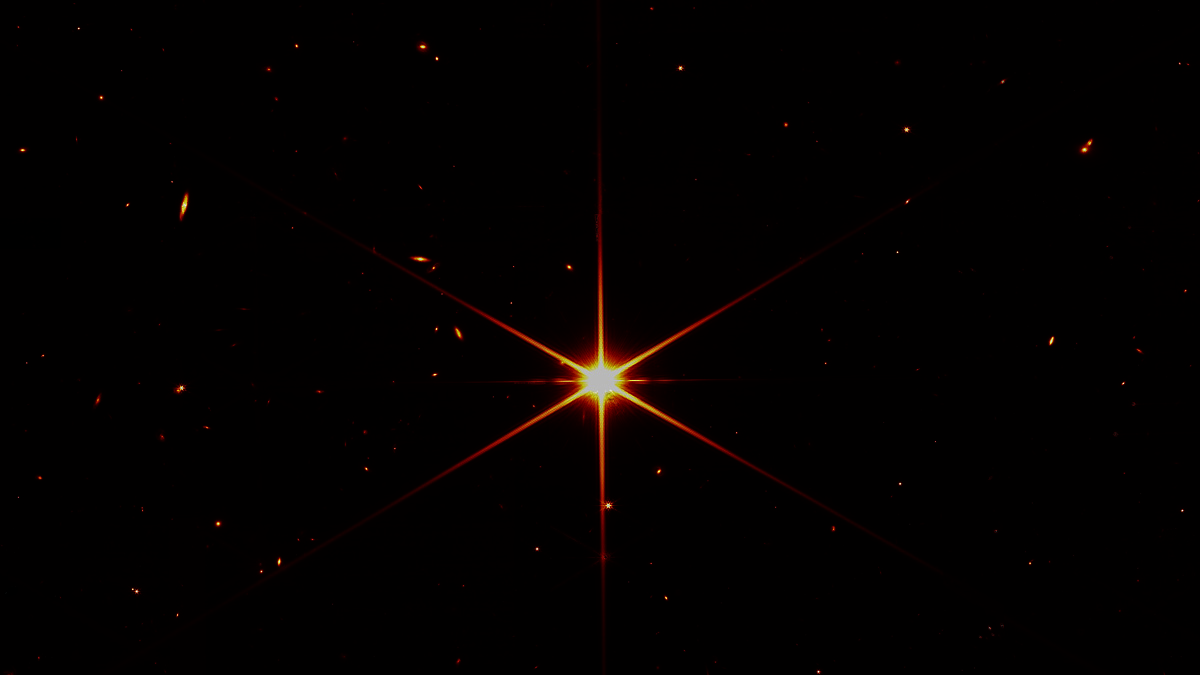
\includegraphics[width=\linewidth]{images/webb.png}
        \caption{Original}
    \end{subfigure}
    \begin{subfigure}[h]{.9\linewidth}
        \centering
        \includegraphics[width=\linewidth]{build/output/webb_mag_n.png}
        \caption{Fourier Transform Magnitude}
        \label{subfig:ftm_n}
    \end{subfigure}
    \begin{subfigure}[h]{.9\linewidth}
        \centering
        \includegraphics[width=\linewidth]{build/output/webb_phase_n.png}
        \caption{Fourier Transform Phase}
        \label{subfig:ftp_n}
    \end{subfigure}
    \begin{subfigure}[h]{.9\linewidth}
        \centering
        \includegraphics[width=\linewidth]{build/output/webb_mag_log.png}
        \caption{Fourier Transform magnitude in logarithmic space}
        \label{subfig:ftm_log}
    \end{subfigure}
    \begin{subfigure}[h]{.9\linewidth}
        \centering
        \includegraphics[width=\linewidth]{build/output/webb_mag.png}
        \caption{FT Magnitude in logarithmic space and rearranged}
        \label{subfig:ftm}
    \end{subfigure}
    \caption{An example of the Fourier transform. The image is the first calibration picture of the new James-Webb space telescope. }
    \label{fig:fourier_example_n}
\end{figure}

As you can see in the example image, the Fourier magnitude is mostly black, and the phases appear to be noise to the eye.
To better distinguish small features, we will now switch to logarithmic color-space for the magnitude
\begin{equation}
    \abs {X''_{k,l,c}} = 255\frac{\log \abs {X_{k,l,c}}-\min_{n,m} \log\abs {X_{n,m,c}} } {\max_{n,m} \log\abs {X_{n,m,c}}-\min_{n,m} \log\abs {X_{n,m,c}}}.
\end{equation}
This is depicted in \autoref{subfig:ftm_log}.
Finally, to better resemble the symmetries in the Fourier space and
to have low frequencies in the middle of the picture, and high frequencies outside,
the indices are shifted
\begin{equation}
    k' = \lfloor k+h/2\rfloor \mod h \qquad l'=\lfloor l+w/2\rfloor\mod w.
\end{equation}
This will be our method of visualization from now on and can be seen in \autoref{subfig:ftm}.

\subsection{Editing in Fourier Space}
If we now modify the numbers in the Fourier space and transform the modified numbers back,
we can achieve complex-looking outcome.
For example, if we take the high frequencies in the image away, we are only left with the
"long-range" information, but the "short-range" information is lost.
This means the image will appear to be blurred.
Taking away the high frequencies can be done in multiple ways.
We can just remove the highest frequencies combining the axes by calculating
$(k'-h/2)^2+(l'-w/2)^2 < r^2$ for some $r$ and setting the pixel in Fourier space to 0, if
this evaluates to false. We can also do this for each axis independently
($(k'-h/2)^2<r_y^2$, $(l'-w/2)^2<r_x^2$).
With these hard cut-offs it is easy to see periodic artifacts in the image.
If we do not want that, we can apply a smooth filter.
A selection of different blurring techniques can be seen
in \autoref{fig:blur_2} to \autoref{fig:blur_smooth}.

\begin{figure}[htbp]
    \centering
    \begin{subfigure}[h]{.49\linewidth}
        \centering
        \includegraphics[width=.9\linewidth]{build/output/dune_mag.png}
        \caption{Fourier space}
    \end{subfigure}
    \begin{subfigure}[h]{.49\linewidth}
        \centering
        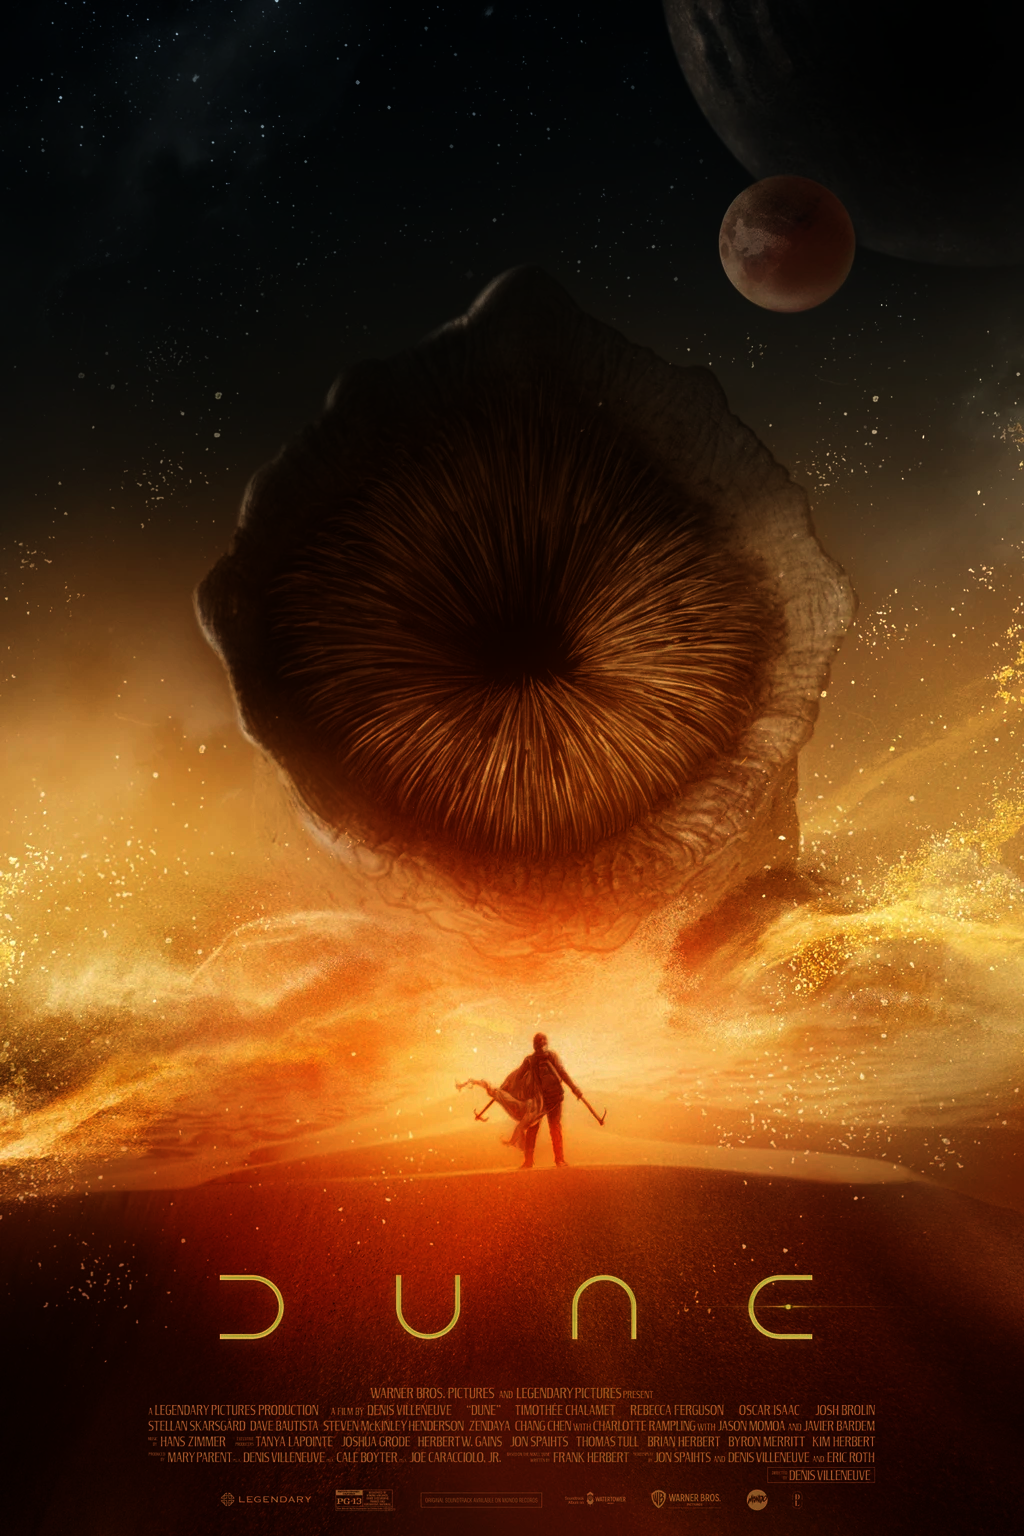
\includegraphics[width=.9\linewidth]{images/dune.png}
        \caption{Original}
    \end{subfigure}\
    \caption{The movie poster of Dune (2021) which serves as an example image being blurred in this section.}
    \label{fig:dune_orig}
\end{figure}

\begin{figure}[htbp]
    \centering
    \begin{subfigure}[h]{.49\linewidth}
        \centering
        \includegraphics[width=.9\linewidth]{build/output/dune_blur2_mask.png}
        \caption{Edit in Fourier space }
    \end{subfigure}
    \begin{subfigure}[h]{.49\linewidth}
        \centering
        \includegraphics[width=.9\linewidth]{build/output/dune_blur2.png}
        \caption{Transformed back to real space}
    \end{subfigure}\
    \caption{The poster above blurred by only keeping the innermost frequencies with a radius of $20\%$ of the width.}
    \label{fig:blur_2}
\end{figure}
\begin{figure}[htbp]
    \centering
    \begin{subfigure}[h]{.49\linewidth}
        \centering
        \includegraphics[width=.9\linewidth]{build/output/dune_blur1_mask.png}
        \caption{Edit in Fourier space }
    \end{subfigure}
    \begin{subfigure}[h]{.49\linewidth}
        \centering
        \includegraphics[width=.9\linewidth]{build/output/dune_blur1.png}
        \caption{Transformed back to real space}
    \end{subfigure}\
    \caption{The poster blurred by only keeping the innermost frequencies with a radius of $10\%$ of the width. This is a circular filter.}
    \label{fig:blur_2}
\end{figure}
\begin{figure}[htbp]
    \centering
    \begin{subfigure}[h]{.49\linewidth}
        \centering
        \includegraphics[width=.9\linewidth]{build/output/dune_rect_mask.png}
        \caption{Edit in Fourier space }
    \end{subfigure}
    \begin{subfigure}[h]{.49\linewidth}
        \centering
        \includegraphics[width=.9\linewidth]{build/output/dune_blur_rect.png}
        \caption{Transformed back to real space}
    \end{subfigure}\
    \caption{The poster blurred by only keeping the $10\%$ innermost frequencies along each axis independently. This is a rectangular filter.}
    \label{fig:blur_rect}
\end{figure}
\begin{figure}[htbp]
    \centering
    \begin{subfigure}[h]{.49\linewidth}
        \centering
        \includegraphics[width=.9\linewidth]{build/output/dune_blur_smooth_mask.png}
        \caption{Edit in Fourier space }
    \end{subfigure}
    \begin{subfigure}[h]{.49\linewidth}
        \centering
        \includegraphics[width=.9\linewidth]{build/output/dune_blur_smooth.png}
        \caption{Transformed back to real space}
    \end{subfigure}\
    \caption{The poster blurred by only multipliying each pixel in the Fourier space with $\exp(-0.001 ((k'-h/2)^2+(l'-w/2)^2))$, where $k', l'$ are the shifted indices from above. This is a Gaussian filter.}
    \label{fig:blur_smooth}
\end{figure}


If we do the opposite and take away some low frequencies, we are sharpening the image.
If we take it to the extreme and remove most low frequencies, we have edge detection.
\begin{figure}[htbp]
    \centering
    \begin{subfigure}[h]{.49\linewidth}
        \centering
        \includegraphics[width=.9\linewidth]{build/output/blackhole_sharp_smooth_mask.png}
        \caption{Fourier space}
    \end{subfigure}
    \begin{subfigure}[h]{.49\linewidth}
        \centering
        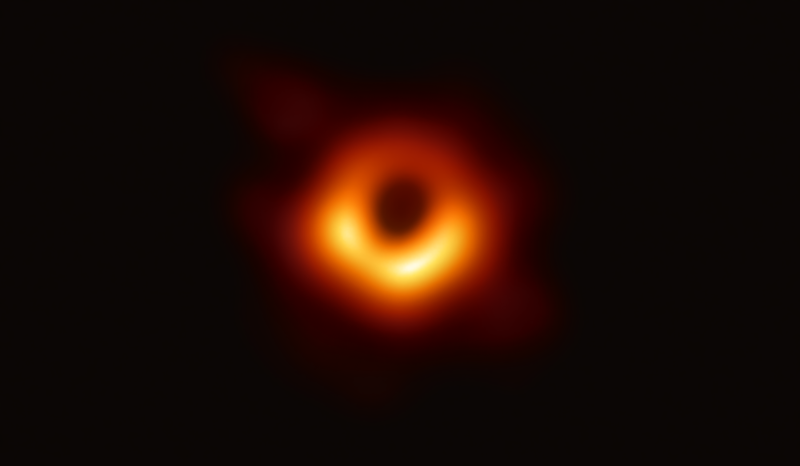
\includegraphics[width=.9\linewidth]{images/blackhole.png}
        \caption{Original}
    \end{subfigure}\
    \caption{The movie poster of Dune (2021) which serves as an example image being blurred in this section.}
    \label{fig:dune_orig}
\end{figure}

\begin{frame}{Thanks for Listening!}
    \printbibliography
\end{frame}

\end{document}

